%%%%%%%%%%%%%%%%%%%%%%%%%%%%% Define Article %%%%%%%%%%%%%%%%%%%%%%%%%%%%%%%%%%
\documentclass{article}
%%%%%%%%%%%%%%%%%%%%%%%%%%%%%%%%%%%%%%%%%%%%%%%%%%%%%%%%%%%%%%%%%%%%%%%%%%%%%%%

%%%%%%%%%%%%%%%%%%%%%%%%%%%%% Using Packages %%%%%%%%%%%%%%%%%%%%%%%%%%%%%%%%%%
\usepackage{geometry}
\usepackage{graphicx}
\usepackage{amssymb}
\usepackage{amsmath}
\usepackage{amsthm}
\usepackage{empheq}
\usepackage{mdframed}
\usepackage{booktabs}
\usepackage{lipsum}
\usepackage{graphicx}
\usepackage{color}
\usepackage{psfrag}
\usepackage{pgfplots,tikz}
\usepackage{bm}
\usepackage{minted}
\usepackage{tikz-3dplot}
\usetikzlibrary{shapes.geometric}
\usetikzlibrary {intersections}
\usetikzlibrary {datavisualization.formats.functions}
\usepackage[svgnames]{xcolor}
%%%%%%%%%%%%%%%%%%%%%%%%%%%%%%%%%%%%%%%%%%%%%%%%%%%%%%%%%%%%%%%%%%%%%%%%%%%%%%%

% Other Settings

%%%%%%%%%%%%%%%%%%%%%%%%%% Page Setting %%%%%%%%%%%%%%%%%%%%%%%%%%%%%%%%%%%%%%%
\geometry{a4paper}

%%%%%%%%%%%%%%%%%%%%%%%%%% Define some useful colors %%%%%%%%%%%%%%%%%%%%%%%%%%
\definecolor{ocre}{RGB}{243,102,25}
\definecolor{mygray}{RGB}{243,243,244}
\definecolor{deepGreen}{RGB}{26,111,0}
\definecolor{shallowGreen}{RGB}{235,255,255}
\definecolor{deepBlue}{RGB}{61,124,222}
\definecolor{shallowBlue}{RGB}{235,249,255}
%%%%%%%%%%%%%%%%%%%%%%%%%%%%%%%%%%%%%%%%%%%%%%%%%%%%%%%%%%%%%%%%%%%%%%%%%%%%%%%

%%%%%%%%%%%%%%%%%%%%%%%%%% Define an orangebox command %%%%%%%%%%%%%%%%%%%%%%%%
\newcommand\orangebox[1]{\fcolorbox{ocre}{mygray}{\hspace{1em}#1\hspace{1em}}}
%%%%%%%%%%%%%%%%%%%%%%%%%%%%%%%%%%%%%%%%%%%%%%%%%%%%%%%%%%%%%%%%%%%%%%%%%%%%%%%

%%%%%%%%%%%%%%%%%%%%%%%%%%%% English Environments %%%%%%%%%%%%%%%%%%%%%%%%%%%%%
\newtheoremstyle{mytheoremstyle}{3pt}{3pt}{\normalfont}{0cm}{\rmfamily\bfseries}{}{1em}{{\color{black}\thmname{#1}~\thmnumber{#2}}\thmnote{\,--\,#3}}
\newtheoremstyle{myproblemstyle}{3pt}{3pt}{\normalfont}{0cm}{\rmfamily\bfseries}{}{1em}{{\color{black}\thmname{#1}~\thmnumber{#2}}\thmnote{\,--\,#3}}
\theoremstyle{mytheoremstyle}
\newmdtheoremenv[linewidth=1pt,backgroundcolor=shallowGreen,linecolor=deepGreen,leftmargin=0pt,innerleftmargin=20pt,innerrightmargin=20pt,]{theorem}{Theorem}[section]
\theoremstyle{mytheoremstyle}
\newmdtheoremenv[linewidth=1pt,backgroundcolor=shallowBlue,linecolor=deepBlue,leftmargin=0pt,innerleftmargin=20pt,innerrightmargin=20pt,]{definition}{Definition}[section]
\theoremstyle{myproblemstyle}
\newmdtheoremenv[linecolor=black,leftmargin=0pt,innerleftmargin=10pt,innerrightmargin=10pt,]{problem}{Problem}[section]
%%%%%%%%%%%%%%%%%%%%%%%%%%%%%%%%%%%%%%%%%%%%%%%%%%%%%%%%%%%%%%%%%%%%%%%%%%%%%%%

%%%%%%%%%%%%%%%%%%%%%%%%%%%%%%% Plotting Settings %%%%%%%%%%%%%%%%%%%%%%%%%%%%%
\usepgfplotslibrary{colorbrewer}
\pgfplotsset{width=8cm,compat=1.9}
%%%%%%%%%%%%%%%%%%%%%%%%%%%%%%%%%%%%%%%%%%%%%%%%%%%%%%%%%%%%%%%%%%%%%%%%%%%%%%%

%%%%%%%%%%%%%%%%%%%%%%%%%%%%%%% Title & Author %%%%%%%%%%%%%%%%%%%%%%%%%%%%%%%%
\title{Graphs using \LaTeX}
\author{Miskatul Anwar}
\date{\tiny{\today}}
%%%%%%%%%%%%%%%%%%%%%%%%%%%%%%%%%%%%%%%%%%%%%%%%%%%%%%%%%%%%%%%%%%%%%%%%%%%%%%%

\begin{document}
\maketitle
\clearpage

%%%%%%%%%%%%%%%%%%%%%%%%%%%%%%% Example 01 %%%%%%%%%%%%%%%%%%%%%%%%%%%%%%%%%%%%
\begin{minipage}{0.45\textwidth}
	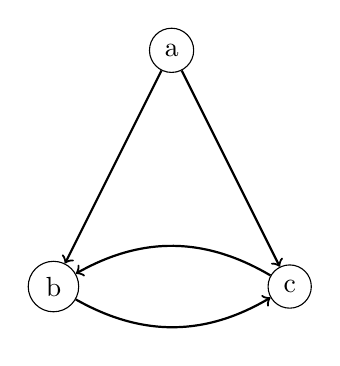
\begin{tikzpicture}[fill=white]
		\path (1.5,3) node(a)[circle, draw , fill]{a}
		(0,0) node(b)[circle, draw, fill]{b}
		(3,0) node(c)[circle, draw, fill]{c};
		\draw [thick, black,->] (a)--(b);
		\draw [thick, black,->] (a)--(c);
		\draw [thick, black,->, bend right=30] (b) to (c);
		\draw [thick, black,->, bend right=30] (c) to (b);
	\end{tikzpicture}
\end{minipage}
\begin{minipage}{0.45\textwidth}
	\begin{minted}[bgcolor=Beige,breaklines,fontsize=\footnotesize]{tex}
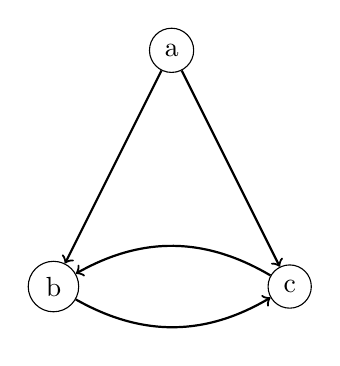
\begin{tikzpicture}[fill=white]
	\path (1.5,3) node(a)[circle, draw , fill]{a}
	(0,0) node(b)[circle, draw, fill]{b}
	(3,0) node(c)[circle, draw, fill]{c};
	\draw [thick, black,->] (a)--(b);
	\draw [thick, black,->] (a)--(c);
	\draw [thick, black,->, bend right=30] (b) to (c);
	\draw [thick, black,->, bend right=30] (c) to (b);
\end{tikzpicture}

\end{minted}
\end{minipage}

\hrule
\begin{minipage}{0.45\textwidth}
	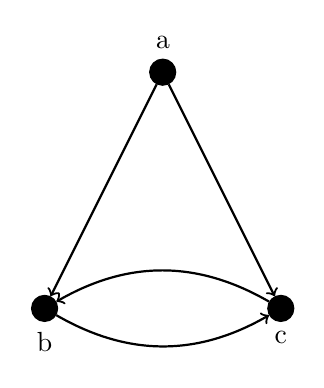
\begin{tikzpicture}[fill=black]
		\path (1.5,3) node(a)[circle, draw , fill,label=a]{}
		(0,0) node(b)[circle, draw, fill,label=below:b]{}
		(3,0) node(c)[circle, draw, fill,label=below:c]{};
		\draw [thick, black,->] (a)--(b);
		\draw [thick, black,->] (a)--(c);
		\draw [thick, black,->, bend right=30] (b) to (c);
		\draw [thick, black,->, bend right=30] (c) to (b);
	\end{tikzpicture}
\end{minipage}
\begin{minipage}{0.45\textwidth}
	\begin{minted}[bgcolor=Beige, breaklines, fontsize=\footnotesize]{tex}
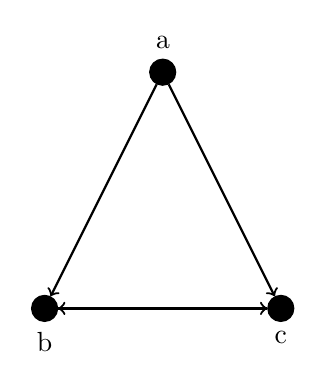
\begin{tikzpicture}[fill=black]
    \path 
        (1.5,3) node(a)[circle, draw, fill, label=a]{}
        (0,0) node(b)[circle, draw, fill, label=below:b]{}
        (3,0) node(c)[circle, draw, fill, label=below:c]{};
    \draw [thick, black, ->] (a) -- (b);
    \draw [thick, black, ->] (a) -- (c);
    \draw [thick, black, ->, bend right=30] (b) --(c);
    \draw [thick, black, ->, bend right=30] (c) --(b);
\end{tikzpicture}
    \end{minted}
\end{minipage}
\hrule
\begin{minipage}{0.45\textwidth}
	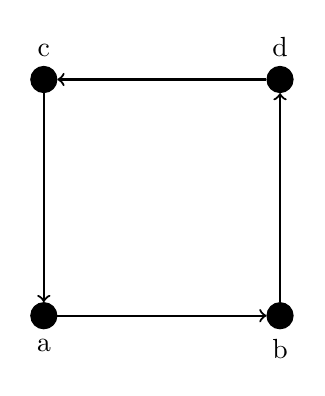
\begin{tikzpicture}[fill=black]
		\path (0,0) node(a)[circle,draw, fill,label=below:a] {}
		(3,0) node(b)[circle,draw, fill,label=below:b] {}
		(0,3) node(c)[circle,draw, fill,label=above:c] {}
		(3,3) node(d)[circle,draw, fill,label=above:d] {};
		\draw[thick,black,->] (a)--(b);
		\draw[thick,black,->] (b)--(d);
		\draw[thick,black,->] (d)--(c);
		\draw[thick,black,->] (c)--(a);
	\end{tikzpicture}
\end{minipage}
\begin{minipage}{0.45\textwidth}
	\begin{minted}[bgcolor=Beige, breaklines, fontsize=\footnotesize]{tex}
	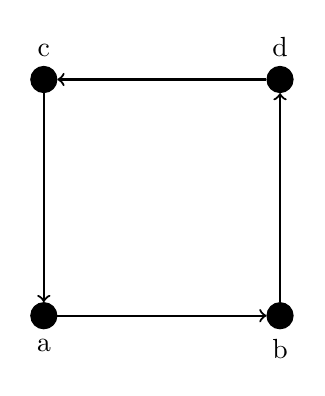
\begin{tikzpicture}[fill=black]
		\path (0,0) node(a)[circle,draw, fill,label=below:a] {}
		(3,0) node(b)[circle,draw, fill,label=below:b] {}
		(0,3) node(c)[circle,draw, fill,label=above:c] {}
		(3,3) node(d)[circle,draw, fill,label=above:d] {};
		\draw[thick,black,->] (a)--(b);
		\draw[thick,black,->] (b)--(d);
		\draw[thick,black,->] (d)--(c);
		\draw[thick,black,->] (c)--(a);
	\end{tikzpicture}
  \end{minted}
\end{minipage}
\newpage
\begin{minipage}{0.45\textwidth}
	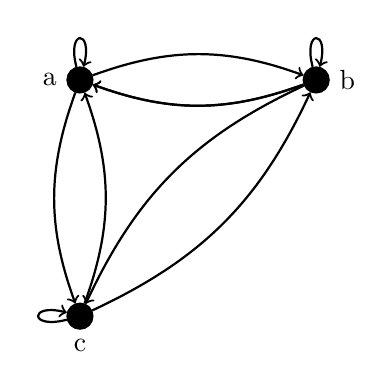
\begin{tikzpicture}
		\path (0,0) node(c)[circle, draw,fill,label=below:c]{}
		(0,3) node(a)[circle,draw,fill,label=left:a]{}
		(3,3) node(b)[circle,draw,fill,label=right:b]{};
		\draw[thick,black,->, bend left=20] (a) to (b);
		\draw[thick,black,->, bend left=20] (b) to (a);
		\draw[thick,black,->, bend left=20] (b) to (a);
		\draw[thick,black,->, bend right=20] (a) to (c);
		\draw[thick,black,->, bend right=20] (c) to (a);
		\draw[thick,black,->, bend right=20] (c) to (b);
		\draw[thick,black,->, bend right=20] (b) to (c);
		\draw[thick,black,->,loop above] (a) to (a);
		\draw[thick,black,->,loop above] (b) to (b);
		\draw[thick,black,->,loop left] (c) to (c);
	\end{tikzpicture}
\end{minipage}
\begin{minipage}{0.7\textwidth}
	\begin{minted}[bgcolor=Beige, breaklines, fontsize=\footnotesize]{tex}
    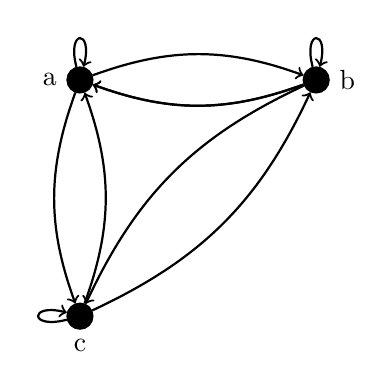
\begin{tikzpicture}[fill=black]
		\path (0,0) node(c)[circle, draw,fill, label=below:c]{}
		(0,3) node(a)[circle,draw,fill, label=left:a]{}
		(3,3) node(b)[circle,draw,fill, label=right:b]{};
		\draw[thick,black,->, bend left=20] (a) to (b);
		\draw[thick,black,->, bend left=20] (b) to (a);
		\draw[thick,black,->, bend left=20] (b) to (a);
		\draw[thick,black,->, bend right=20] (a) to (c);
		\draw[thick,black,->, bend right=20] (c) to (a);
		\draw[thick,black,->, bend right=20] (c) to (b);
		\draw[thick,black,->, bend right=20] (b) to (c);
		\draw[thick,black,->, loop above] (a) to (a);
		\draw[thick,black,->, loop above] (b) to (b);
		\draw[thick,black,->, loop left] (c) to (c);
	
 \end{tikzpicture} 
\end{minted}
\end{minipage}
\hrule
\begin{minipage}{0.45\textwidth}
	\vspace{10mm}
	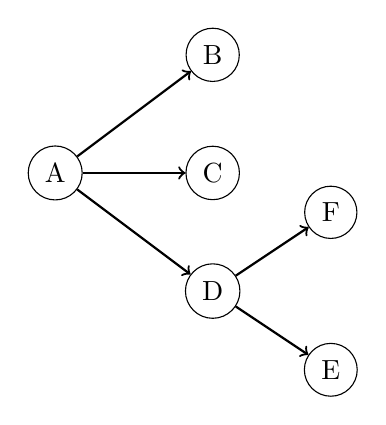
\begin{tikzpicture}[fill=white]
		\path (0,1.5) node(a)[circle,draw,fill]{A}
		(2,3) node(b)[circle,draw,fill]{B}
		(2,1.5)node(c)[circle,draw,fill]{C}
		(2,0)node(d)[circle,draw,fill]{D}
		(3.5,-1) node(e)[circle,draw,fill]{E}
		(3.5,1) node(f)[circle,draw,fill]{F};
		\draw [thick,black,->] (a) to (b);
		\draw [thick,black,->] (a) to (c);
		\draw [thick,black,->] (a) to (d);
		\draw [thick,black,->] (d) to (e);
		\draw [thick,black,->] (d) to (f);
	\end{tikzpicture}
\end{minipage}
\begin{minipage}{0.7\textwidth}
	\begin{minted}[bgcolor=Beige, breaklines, fontsize=\footnotesize]{tex}
	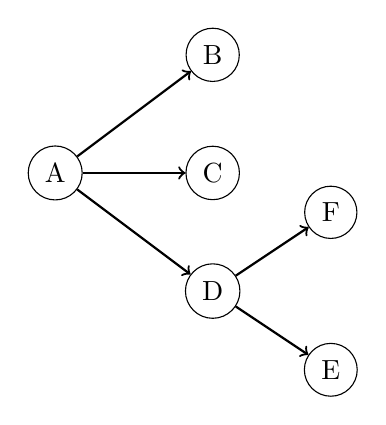
\begin{tikzpicture}[fill=white]
		\path (0,1.5) node(a)[circle,draw,fill]{A}
		(2,3) node(b)[circle,draw,fill]{B}
		(2,1.5)node(c)[circle,draw,fill]{C}
		(2,0)node(d)[circle,draw,fill]{D}
		(3.5,-1) node(e)[circle,draw,fill]{E}
		(3.5,1) node(f)[circle,draw,fill]{F};
		\draw [thick,black,->] (a) to (b);
		\draw [thick,black,->] (a) to (c);
		\draw [thick,black,->] (a) to (d);
		\draw [thick,black,->] (d) to (e) ;
		\draw [thick,black,->] (d) to (f);
	\end{tikzpicture}
\end{minted}
\end{minipage}
\hrule
\vspace{1mm}
\begin{minipage}{0.45\textwidth}
	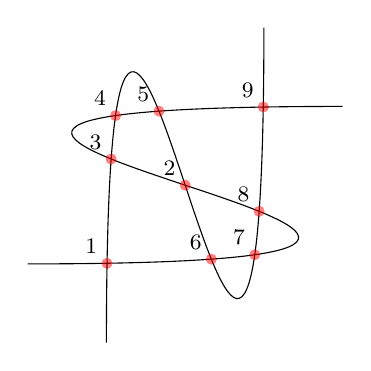
\begin{tikzpicture}
		\clip (-2,-2) rectangle (2,2);
		\draw [name path=curve 1] (-2,-1) .. controls (8,-1) and (-8,1) .. (2,1);
		\draw [name path=curve 2] (-1,-2) .. controls (-1,8) and (1,-8) .. (1,2);
		\fill [name intersections={of=curve 1 and curve 2, name=i, total=\t}]
		[red, opacity=0.5, every node/.style={above left, black, opacity=1}]
		\foreach \s in {1,...,\t}{(i-\s) circle (2pt) node {\footnotesize\s}};
	\end{tikzpicture}
\end{minipage}
\begin{minipage}{0.7\textwidth}
	\begin{minted}[bgcolor=Beige, breaklines, fontsize=\footnotesize]{tex}
	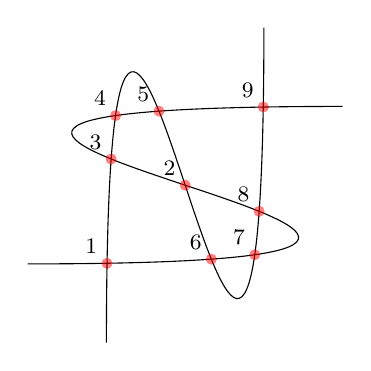
\begin{tikzpicture}
		\clip (-2,-2) rectangle (2,2);
		\draw [name path=curve 1] (-2,-1) .. controls (8,-1) and (-8,1) .. (2,1);
		\draw [name path=curve 2] (-1,-2) .. controls (-1,8) and (1,-8) .. (1,2);
		\fill [name intersections={of=curve 1 and curve 2, name=i, total=\t}]
		[red, opacity=0.5, every node/.style={above left, black, opacity=1}]
		\foreach \s in {1,...,\t}{(i-\s) circle (2pt) node {\footnotesize\s}};
	\end{tikzpicture}
  \end{minted}
\end{minipage}
\hrule
\begin{minipage}{0.4\textwidth}
	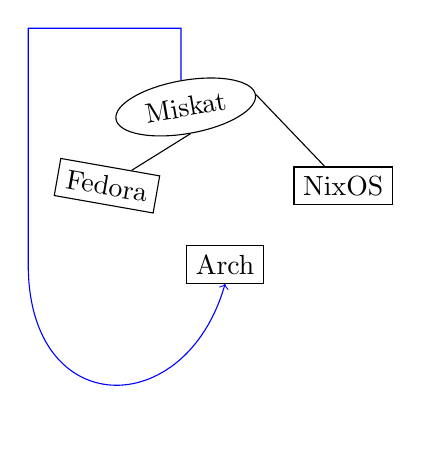
\begin{tikzpicture}[fill=white]
		\path (4,4) node(a)[ellipse,draw,fill,rotate=10]{Miskat}
		(3,3) node(b) [rectangle, draw,fill,rotate=-10]{Fedora}
		(6,3) node(c) [rectangle,draw,fill]{NixOS}
		(4.5,2) node(d) [rectangle,draw,fill]{Arch};
		\draw (a.south) -- (b);
		\draw (a.east) -- (c);
		\draw [blue,->](a.north) |-(2,5) -- (2,2) .. controls (2,0)and (4,0) .. (d.south);
	\end{tikzpicture}
\end{minipage}
\begin{minipage}{0.7\textwidth}
	\begin{minted}[bgcolor=Beige,breaklines,fontsize=\footnotesize]{tex}
  	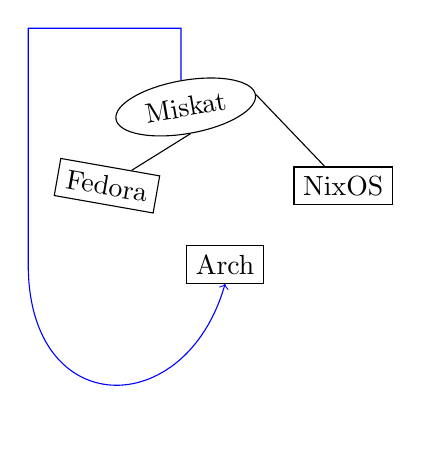
\begin{tikzpicture}[fill=white]
		\path (4,4) node(a)[ellipse,draw,fill,rotate=10]{Miskat}
		(3,3) node(b) [rectangle, draw,fill,rotate=-10]{Fedora}
		(6,3) node(c) [rectangle,draw,fill]{NixOS}
		(4.5,2) node(d) [rectangle,draw,fill]{Arch};
		\draw (a.south) -- (b);
		\draw (a.east) -- (c);
		\draw [blue,->](a.north) |-(2,5) -- (2,2) .. controls (2,0) and (4,0) .. (d.south);
	\end{tikzpicture}
  \end{minted}
\end{minipage}
\hrule
\begin{minipage}

\end{minipage}
\end{document}

